%%%%%%%%%%%%%%%%%%%%%%%%%%%%%%%%%%%%%%%%%
% Stylish Article
% LaTeX Template
% Version 2.1 (1/10/15)
%
% This template has been downloaded from:
% http://www.LaTeXTemplates.com
%
% Original author:
% Mathias Legrand (legrand.mathias@gmail.com) 
% With extensive modifications by:
% Vel (vel@latextemplates.com)
%
% License:
% CC BY-NC-SA 3.0 (http://creativecommons.org/licenses/by-nc-sa/3.0/)
%
%%%%%%%%%%%%%%%%%%%%%%%%%%%%%%%%%%%%%%%%%

%----------------------------------------------------------------------------------------
%	PACKAGES AND OTHER DOCUMENT CONFIGURATIONS
%----------------------------------------------------------------------------------------

\documentclass[fleqn,10pt]{SelfArx} % Document font size and equations flushed left

\usepackage[english]{babel} % Specify a different language here - english by default

\usepackage{lipsum} % Required to insert dummy text. To be removed otherwise
\usepackage{graphicx}
\graphicspath{ {images/} }

%----------------------------------------------------------------------------------------
%	COLUMNS
%----------------------------------------------------------------------------------------

\setlength{\columnsep}{0.55cm} % Distance between the two columns of text
\setlength{\fboxrule}{0.75pt} % Width of the border around the abstract

%----------------------------------------------------------------------------------------
%	COLORS
%----------------------------------------------------------------------------------------

\definecolor{color1}{RGB}{0,0,90} % Color of the article title and sections
\definecolor{color2}{RGB}{0,20,20} % Color of the boxes behind the abstract and headings

%----------------------------------------------------------------------------------------
%	HYPERLINKS
%----------------------------------------------------------------------------------------

\usepackage{hyperref} % Required for hyperlinks
\hypersetup{hidelinks,colorlinks,breaklinks=true,urlcolor=color2,citecolor=color1,linkcolor=color1,bookmarksopen=false,pdftitle={Title},pdfauthor={Author}}

%----------------------------------------------------------------------------------------
%	ARTICLE INFORMATION
%----------------------------------------------------------------------------------------

\JournalInfo{Introduction to Data Analysis  and Mining 2018} % Journal information
\Archive{} % Additional notes (e.g. copyright, DOI, review/research article)

\PaperTitle{Porto Seguro Insurance Claim Prediction} % Article title

\Authors{William Huibregtse\textsuperscript{1}, Joshua Baker\textsuperscript{1}, Chris East\textsuperscript{1}} % Authors
\affiliation{\textsuperscript{1}\textit{Computer Science, School of Informatics , Computing and Engineering, Indiana University, Bloomington, IN, USA}} % Author affiliation


\Keywords{Data Processing --- Naive Bayes --- Gradient Boosing --- Cross Validation --- PCA} % Keywords - if you don't want any simply remove all the text between the curly brackets
\newcommand{\keywordname}{Keywords} % Defines the keywords heading name

%----------------------------------------------------------------------------------------
%	ABSTRACT
%----------------------------------------------------------------------------------------

\Abstract{Predicting driver insurance claim probability in upcoming year. Maintaining variable value distributions while replacing missing values in binary, continuous, and ordinal data. Dimensionality reduction using PCA and scaled variable to unit variances. Gradient boosting and Naive Bayes predictive model training.}

%----------------------------------------------------------------------------------------

\begin{document}

\flushbottom % Makes all text pages the same height

\maketitle % Print the title and abstract box

\tableofcontents % Print the contents section

\thispagestyle{empty} % Removes page numbering from the first page




%----------------------------------------------------------------------------------------
%Problem and Data Description
%----------------------------------------------------------------------------------------


\section{Problem and Data Description} % The \section*{} command stops section numbering




First we want to get a general idea of our data set and get a deeper understanding of the underlying structure.\\
There are 59 named features or variables for our data set. \\
With 892816 observations for training and 595212 for test\\
There are no duplicate observations. \\
Features that belong to similar groupings are given certain feature names.\\
- Ind: related to individual or driver\\
- Reg: related to geographical region\\
- Car: related to car being insured\\
- Calc: are calculated features done by Proto themselves\\
Postfix descriptors describes the features data type.\\
- Bin: Binary (1 or 0)\\
- Cat: Categorical *Note: the dataset has the categorical data already convert into factors and then integers\\
- All other variables are either integer or numeric\\
As stated the Data Types are numeric and integer, with integer being the predominant type 49 to 10.\\
Missing values are represented by -1.\\
In total, there are 13 variables with missing values.\\
There is Target feature which denotes the binary classification for that observation. This feature is the feature we are trying to learn/predict for the test data.\\
There is an ID feature which is an anonymized identities of insured drivers.  \\

Porto Seguro’s Safe Driver Prediction has 59 variables and 1.3 million observations, which qualifies as a good candidate for reducing overall dimensions of the data to significantly increase the speed of analysis techniques at the cost of more upfront data processing.


There are only 21694 cases of classification 1, which is 3.64 percent of the observations in the training data set, showing significant skew in the expected class towards a ``0'' prediction.


\bigskip
\bigskip

%----------------------------------------------------------------------------------------
%	Data Preprocessing $\&$ Exploratory Data Analysis
%----------------------------------------------------------------------------------------

\section{Data Preprocessing $\&$ Exploratory Data Analysis} % The \section*{} command stops section numbering

\subsection{Feature Engineering}
Originally, we attempted to feature engineer a new variable of the count of missing values for each entry, but was later decided to be removed as we improved missing value handling to a point where keeping track of countsr of missing values was uneccessary.
\subsection{Handling Missing Values}
\textbf{Overview of features with missing entries}\\
An important aspect of data preprocessing is handling missing data. In total, there are 13 features that have at least 1 missing value. For both the training ($Table 1.$) and testing ($Table 2.$) data the individual features are broken down into: number of missing entries, and percentage of total entries that are missing. As the tables show, both training and training have extremely close value for all the features. The next step is comparing the distribution of features with missing entries between training and testing.\\  
Taking a look at the graphs located in the $Appendix$ we see that all the features have incredible close distribution between Training and Testing, for the exception of $ps-car-12$. However, this feature has 1 missing entry in Training and 0 in Testing. Therefore, the difference in this feature should be ignored. The importance of both distribution and number of missing entries being extremely close is that the methodology developed to handle NA's in Training is applicable for Testing. \\
\\


\begin{table}[ht]
\caption{Train features with missing values} % title of Table
\centering % used for centering table
\begin{tabular}{c c c } % centered columns (4 columns)
\hline\hline %inserts double horizontal lines
Feature & Train & \% Missing\\ [0.5ex] % inserts table
%heading
\hline % inserts single horizontal line
$ps-ind-02-cat$ & 216 & 0.036\\
$ps-ind-04-cat$ & 83 & 0.014\\
$ps-ind-05-cat$ & 5809 & 0.98\\
$ps-reg-03$ & 107772 & 18.11\\
$ps-car-01-cat$ & 107 & 0.018\\
$ps-car-02-cat$ & 5 & 0.001\\
$ps-car-03-cat$ & 411231 & 69.09\\
$ps-car-05-cat$ & 266551 & 44.78\\
$ps-car-07-cat$ & 11489 & 1.93\\
$ps-car-09-cat$ & 569 & 0.10\\
$ps-car-11$ & 5 & 0.001\\
$ps-car-12$ & 1 & 0.0002\\
$ps-car-14$ & 42620 & 7.160474\\ [1ex] % [1ex] adds vertical space
\hline %inserts single line
\end{tabular}
\label{table:nonlin} % is used to refer this table in the text
\end{table}
\begin{table}[ht]
\caption{Test features with missing values } % title of Table
\centering % used for centering table
\begin{tabular}{c c c} % centered columns (4 columns)
\hline\hline %inserts double horizontal lines
Feature & Test & \% Missing \\ [0.5ex] % inserts table
%heading
\hline % inserts single horizontal line
$ps-ind-02-cat$ & 307 & 0.034\\
$ps-ind-04-cat$ & 145 & 0.016\\
$ps-ind-05-cat$ & 8710 & 0.97\\
$ps-reg-03$ & 161684 & 18.11\\
$ps-car-01-cat$ & 160 & 0.018\\
$ps-car-02-cat$ & 5 & 0.001\\
$ps-car-03-cat$ & 616911 & 69.10\\
$ps-car-05-cat$ & 400359 & 44.84\\
$ps-car-07-cat$ & 17331 & 1.94\\
$ps-car-09-cat$ & 877 & 0.10\\
$ps-car-11$ & 1 & 0.0001\\
$ps-car-12$ & 0 & 0\\
$ps-car-14$ & 63805 & 7.15\\ [1ex] % [1ex] adds vertical space
\hline %inserts single line
\end{tabular}
\label{table:nonlin} % is used to refer this table in the text
\end{table}
\newpage
\textbf{Handling missing entries}\\
The features with missing entries are a mixture of categorical with binary or several factors, and then continuous values between 0 and 1. This mixture requires a different approach for each feature.\\\\
\textit{Features with high percentage of missing values:}\\
\\
Two main features stick out: $ps-car-03-cat$ and $ps-car-05-cat$ . With 69\% and 44.8\% missing entries respectively. Both features are binary categorical variables describing the car that's being insured. Given the fact this is a binary variable that describes the car and that there's an overwhelming percentage of missing values we thought it might be best to delete these features. As a quick check before we remove them, we examine the percentage of missing values with the target value of 1 vs the number of total claims (target value = 1). Surprisingly, $ps-car-03-cat$ feature with 69.1\% of it's entries missing with the target 1 accounts for 62\% of the total claims! Same goes for $ps-car-05-cat$  feature with 44.8\% of it's entries missing with the target 1 accounts for 39\% of the total claims! Here it seems that the value missing can be an important feature in predicting claims. Therefore, we replace -1 with 2 and set NA's to their own category. Changing the binary value to an ordinal to preserve the no response characteristic of our data. $Note:$ 2 was decided vs -1 to remove the negative value
\textit{Other Categorical Features with low percentage of missing values:}\\
\\
All of these features are categorical, with low \% of missing entries \(< 2\%\) and mainly very low \% missing entry claim vs total claim. Therefore, we can treat these features as discrete random variables. Which allows us to replace these missing values from a probability density function model after the non-missing entries in each feature. The important goal here is to not alter the distribution of the non-missing values. \\
\\
\textbf{Example:} ps-ind-05-cat\\
Below is an example of the effects of using a PDF based on the probabilities of the non-missing entries to draw replacement values.
\newpage
This is the histogram of the values for ps-ind-05-cat, clearly there are a few -1 values. It also shows the general distribution of the other categorical values for this feature.\\ 
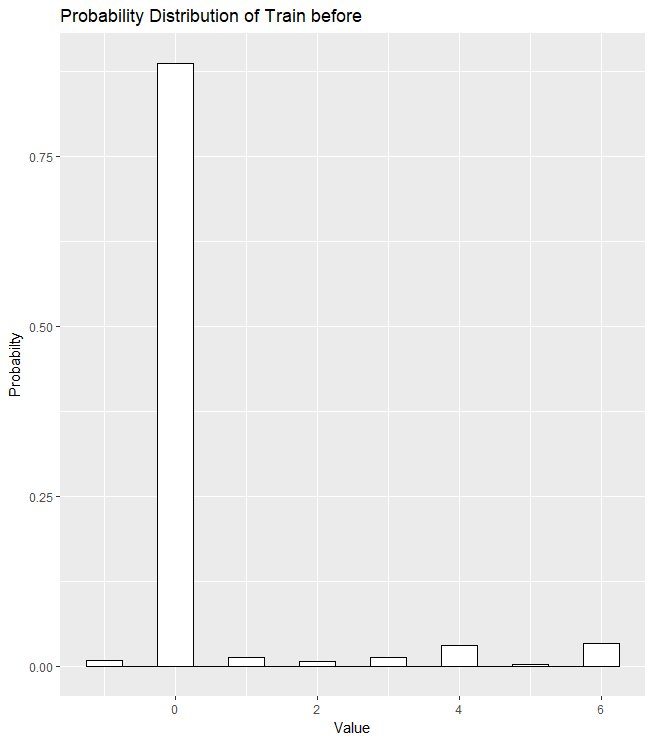
\includegraphics[width=8cm, height=10cm]{ex_before} \\
\\
This is a plot of the new values generate to replace the missing entries based on the distribution of the non-missing entries for the feature. This plot clearly shows that the distribution of the non-missing entries is retained in these new values.\\
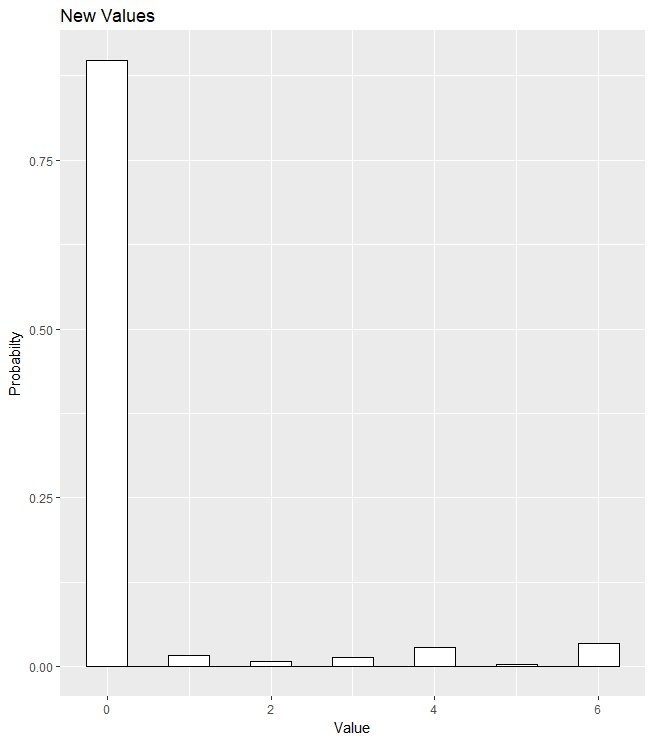
\includegraphics[width=8cm, height=9cm]{ex_new} \\
\newpage
This is the plot of the values after replacing. We see that there are no longer -1 entries, and that the overall distribution has changed very little.\\
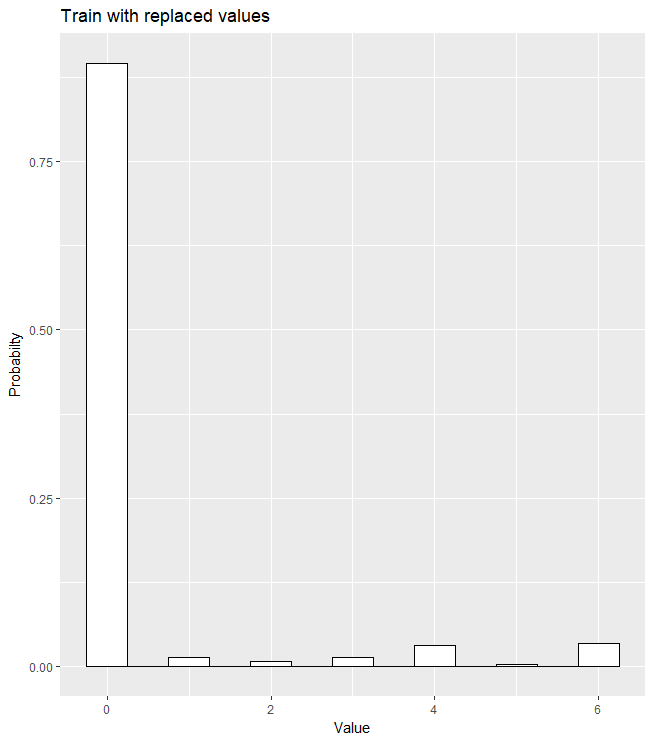
\includegraphics[width=8cm, height=10cm]{ex_finished} \\
\\ This method is applied to 6 categorical features: ps-car-01-cat, ps-car-07-cat, ps-car-09-cat, ps-ind-02-cat, ps-ind-04-cat, and ps-ind-05-cat \\
\\
\textit{Features with continuous distributions between 0 and 1:}\\
\\
There is a single continuous feature: ps-car-14. This feature has a low number of missing entries (7.2\%) and a low \% of missing that are a claim vs total claim (7.9\%), making this a good candidate to replace missing entries with values drawn from a Continuous Random Variable.\\
Here the feature's non-missing entries has a log-normal distribution. Therefore, we'll use $rlnorm$ to approximate the distribution when drawing replacement values.\\
\newpage
This is the histogram of the values for ps-car-14, clearly there are a few -1 values. It also shows the general distribution of the other continuous values for this feature.\\ 
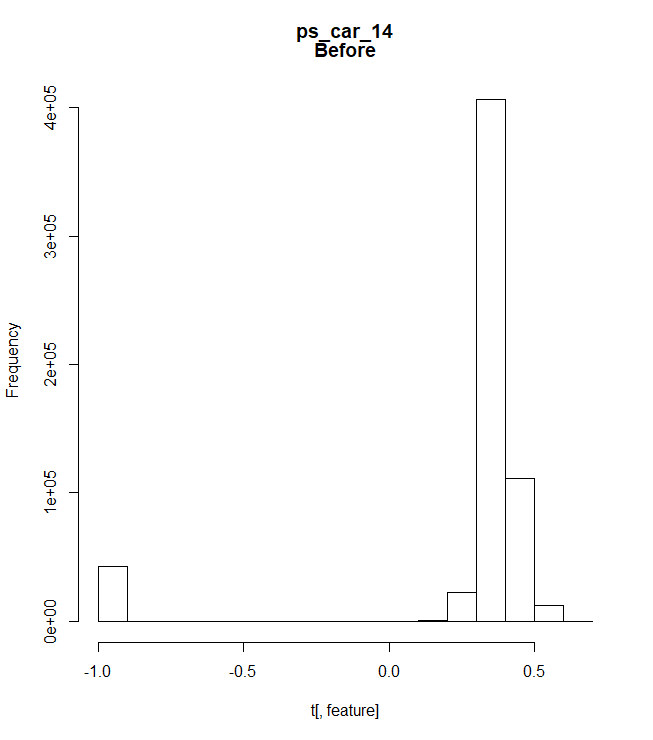
\includegraphics[width=8cm, height=8cm]{cont-before} \\
\\
This is the histogram of the non-missing values for ps-car-14, showing the true distribution of the continuous values for this feature.\\ 
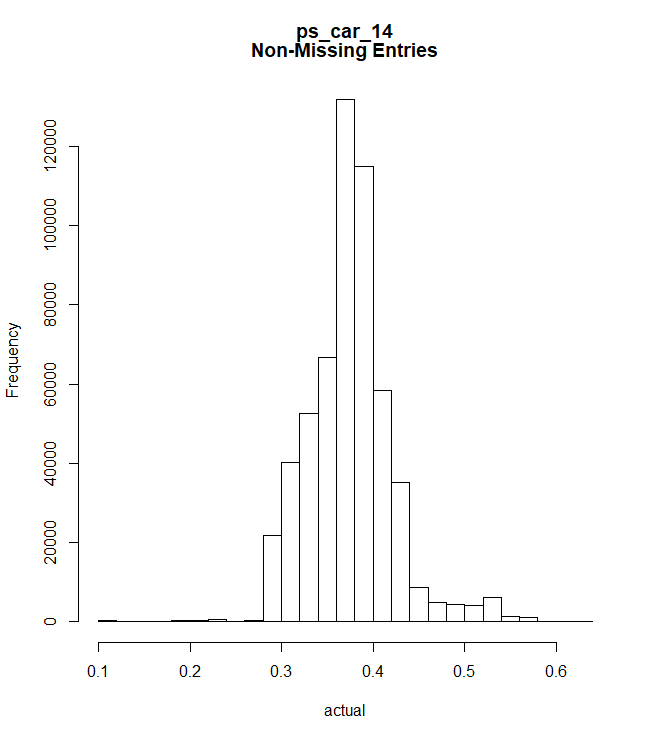
\includegraphics[width=8cm, height=8cm]{cont-actual} \\
\newpage
This is the histogram of the non-missing values plus the density curve for the log-normal pdf we generated from the distribution of the non-missing entries. As shown, the pdf has a good fit and allows for us to draw from it to replace missing entries for the ps-car-14 feature.\\ 
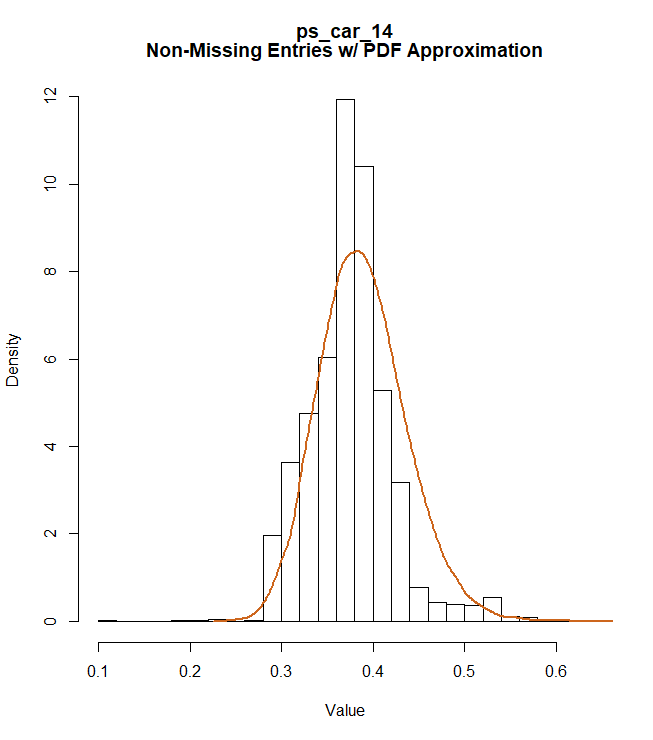
\includegraphics[width=8cm, height=8cm]{cont-pdf} \\
\\
This is the final histogram of the feature with the missing entries replaced. We can see that the overall distribution is intact.\\ 
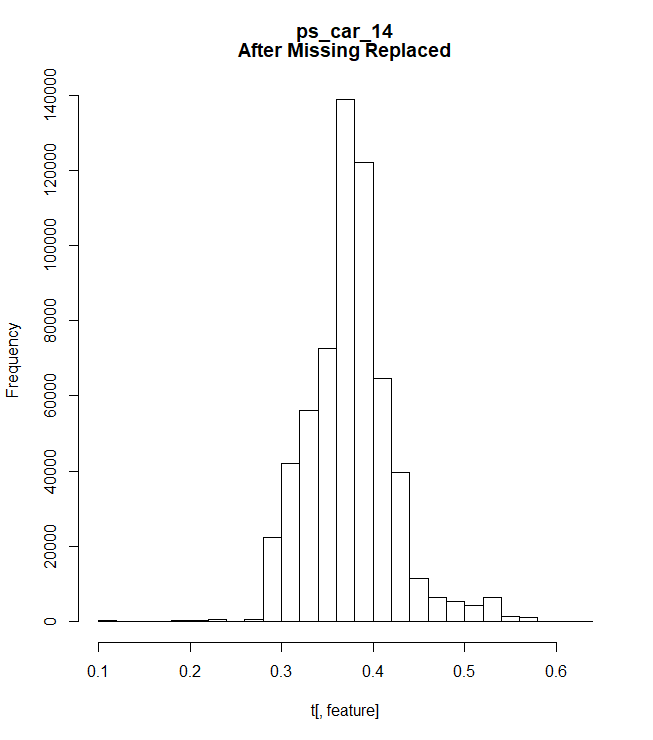
\includegraphics[width=8cm, height=8cm]{cont-after} \\
\newpage
\textit{Features with extremely few missing entries}\\
\\
The rest of the features have an extreme small number of missing entries \(<5\). Therefore, we simply replace the missing entries with the mode of the feature. This is a more than adequate approach for so few observations in our data set (nearly 0\%). \\

\subsection{Exploratory Data Analysis}

Originally, after looking through a few useful posts about PCA on the Kaggle discussion boards about the number of principal components to include in dimensionality reduction, one popular post used PCA without scaling to form new components. This is likely a poor decision as the variables in the data have vastly different variances and ranges, even though all are numerical. To perform PCA on this data, the built in scaling parameter was used to force all variables into unit variances so that each variable was treated with equal weight in PCA. The discussion post in question found that 95 percent of variance was captured within the first 15 principle components when using unscaled data, however our findings show that 95 percent of variance is not captured within the new data until the first 45 are considered, thus PCA would only be reducing the variable size from 57 to 45, which is only a 20 percent reduction in overall dimensions. When moving on to later steps in analysis, the change in variables to unit variances was kept, however no components were dropped as the majority of components needed to be considered before an appropriately large proportion of overall variance was achieved.

Note: To perform this transformation correctly, the test and train data must be transformed together and split after the dimensions have been reduced.
\bigskip
\bigskip
%----------------------------------------------------------------------------------------
 % Algorithm and Methodology
%----------------------------------------------------------------------------------------


\section{Algorithm and Methodology}


\subsection{Naive Bayes}
Once the data was processed, we used the Naive Bayes algorithm to form our model. We tested it with both the implementation from the e1071 package and the caret package. The caret package implementation ended up being more powerful since it allowed for easy cross validation. 

Our analysis with the Naive Bayes algorithm uses the m-estimate smoothing technique to avoid conditional probabilities of 0, however none of the conditional probabilities found were 0, so this added layer of protection was not necessary in this case, likely due to the very large data size. The formula for Naive Bayes is as follows:
\begin{equation}
\label{eq:bayes}
P(\theta|\textbf{D}) = P(\theta ) \frac{P(\textbf{D} |\theta)}{P(\textbf{D})}
\end{equation}
The algorithm gives the probability of an outcome based on a set of conditions from each condition’s probability of individually implying the outcome.

\subsection{Gradient Boosting}
We wanted to test a second classifier, so we chose gradient boosting, since it had been used successfully by a number of people previously. The algorithm tries to minimize a loss function with gradient descent, using progressively smaller learning rates. In order to do this it uses multiple decision trees trained on the data set, each with a different weight that can be updated in the gradient descent step. By using multiple decision trees, the chance of over- fitting to the training data is reduced significantly. By sequentially updating them with gradient descent, the trees further learn from the mistakes of previous trees, so this helps further increase accuracy. 

We used the xgboost R package, which is a popular and fast R package for gradient boosting. The binary logistic regression objective automatically outputs the probability, which worked well for our purposes. It ran significantly faster than Naive Bayes, meaning we were able to test a number of different learning rates, tree depths, and max iterations. The function has built- in error evaluation, which was helpful for deciding what parameters to use. 

\bigskip
\bigskip
%----------------------------------------------------------------------------------------
 % Experiments and Results
%----------------------------------------------------------------------------------------
\section{Experiments and Results}
Our original, crude method of replacing missing values was done by using the mean of each variable. This yielded a maximum score of 0.20566 using Naive Bayes. Using our more advanced techniques to replace these values, we acheived 0.21716 using an XGBoost model. Our XGBoost technique was significantly faster to run, and received our highest score. The Naive bayes technique acheived a score of 0.20090, meaning the improved missing value handling seemed to have little to no effect on performance.


%Upon completing the first predictions against the autograding tool on Kaggle, different sizes of highest variance principle components were tested to see the effect on overall GINI score. A jump from 0.125 to 0.20 was achieved by including the first 16 principle components versus originally using just 5 (99 versus 95 percent of total variance represented in each sample, respectively). %

\bigskip
\bigskip
%----------------------------------------------------------------------------------------
 % Summary and Conclusions
%----------------------------------------------------------------------------------------
\section{Summary and Conclusions}
Overall, a Normalized Gini score of 0.21716 is not good enough to be a top score from Kaggle. The best predictions in the competition used nerual net techniques mixed with gradient boosting for their data analysis. Although the technique of xgboost was common in top finishers, it was often combined with other techniques to form better predictions than ours. Our techniques for replacing missing values is fairly robust, where new values very closely represent the distribution of their variable, however, there may have been correlation or other relationship-based techniques to replace data in a way that maintains relationships between variables that is not simply randomly replacing values while maintaining the distribution for the variable as this method would likely decrease any relationships between variables, which is not ideal.
\bigskip
\bigskip
\bigskip

\section{Appendix}
\subsection{Missing Values}
Plotting the distribution of features with missing values: Training \& Testing\\
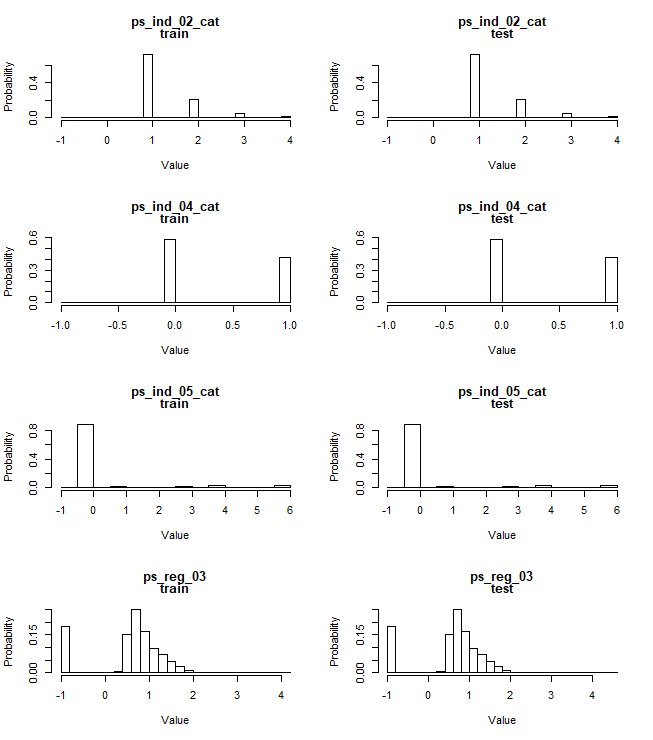
\includegraphics[width=8cm, height=10cm]{comp_1} \\
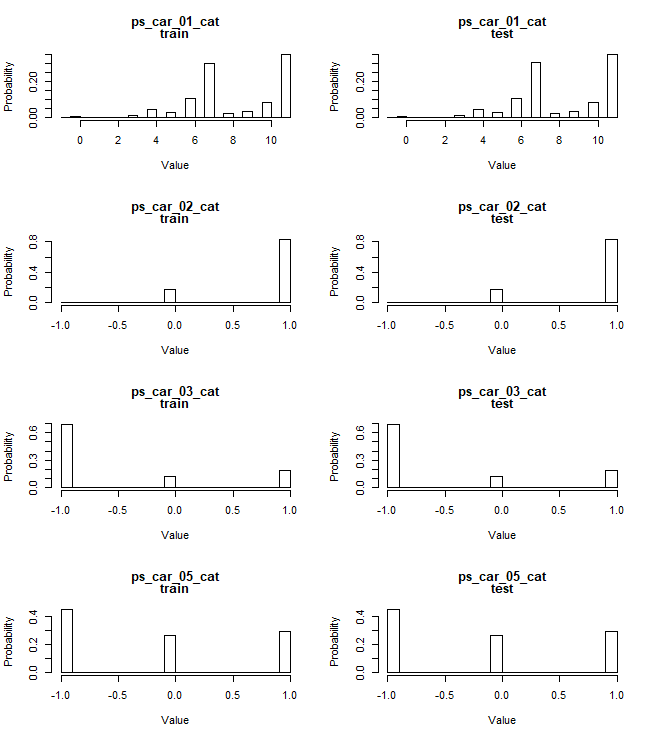
\includegraphics[width=8cm, height=10cm]{comp_2} \\
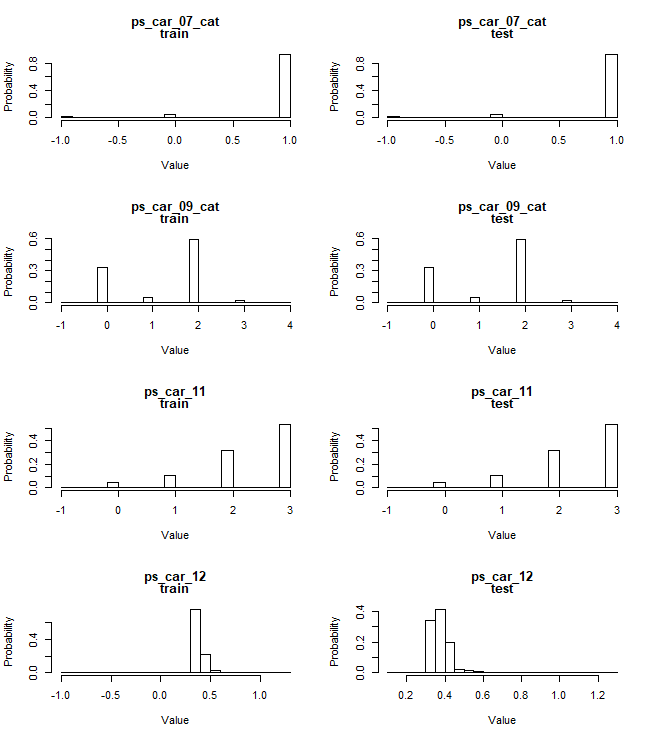
\includegraphics[width=8cm, height=10cm]{comp_3} \\
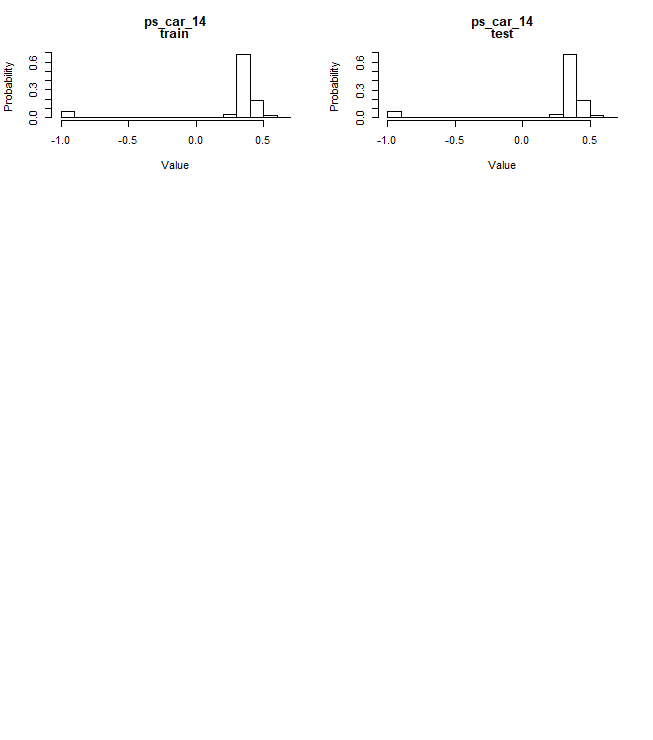
\includegraphics[width=8cm, height=3cm]{comp_4} \\

\phantomsection
\section*{Acknowledgments} % The \section*{} command stops section numbering
\subsection{R packages}


ggplot2\\
caret\\
e1071\\
xgboost
\addcontentsline{toc}{section}{Acknowledgments} % Adds this section to the table of contents



%----------------------------------------------------------------------------------------
%	REFERENCE LIST
%----------------------------------------------------------------------------------------
\phantomsection
\bibliographystyle{unsrt}
\bibliography{sample}

%----------------------------------------------------------------------------------------

\end{document}